\section{Classifying by Determinant}
\begin{frame}{THC-cromwell matrix}
	\begin{itemize}
		\item The \term{THC-cromwell matrix} is an expansion of cromwell matrix into $\theta$-curves and handcuff graphs
	\end{itemize}
	\vspace{1cm}
	\begin{tabu}{X[5c]X[c]X[5c]}
		\raisebox{-1.5cm}{
\includegraphics[height=3cm]{figure/excromwell.png}} &			
		$\longmapsto$ &
		\raisebox{-1.5cm}{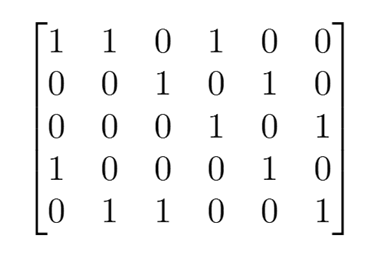
\includegraphics[height=3cm]{figure/cromwell.png}} &
	\end{tabu}
	
\end{frame}

\begin{frame}{Determinant of the cromwell matrices of Knot}
	\begin{thm}
		Let $K$ be any knot then its determinant of the cromwell matrix is $0$ or $\pm2$.
	\end{thm}
	\mypf
	\begin{tabu}{X[5c]X[2c]X[5c]X[c]X[2c]}
			\raisebox{-1.5cm}{\includegraphics[height=3cm]{trefoilimage.png}} &
			$\xmapsto{\text{grid diagram}}$ &
			\raisebox{-1.5cm}{
\includegraphics[height=3cm]{figure/gridtheta.png}} &
			$\xmapsto{THC-cromwell}$ &
	\end{tabu}
	\begin{tabu}{X[c]X[1.5c]X[5c]X[c]X[5c]}
			\raisebox{-1.5cm}{
\includegraphics[height=3cm]{figure/white.png}} &
			$\xmapsto{THC-cromwell}$ &
			$\begin{bmatrix}
				\textcolor{red}{1} & 0 & \textcolor{red}{1} & 0 & 0\\
				0 & \textcolor{red}{1} & 0 & \textcolor{red}{1} & 0\\
				0 & 0 & \textcolor{red}{1} & 0 & \textcolor{red}{1}\\
				\textcolor{red}{1} & 0 & 0 & \textcolor{red}{1} & 0\\
				0 & \textcolor{red}{1} & 0 & 0 & \textcolor{red}{1}
			\end{bmatrix}$&
			$\xmapsto[operations]{row/column}$ &
			$\begin{bmatrix}
				\textcolor{red}{1} & \textcolor{red}{1} & 0 & 0 & 0\\
				0 & \textcolor{red}{1} & \textcolor{red}{1} & 0 & 0\\
				0 & 0 & \textcolor{red}{1} & \textcolor{red}{1} & 0\\
				0 & 0 & 0 & \textcolor{red}{1} & \textcolor{red}{1}\\
				\textcolor{red}{1} & 0 & 0 & 0 & \textcolor{red}{1}
			\end{bmatrix}$
	\end{tabu}
\end{frame}
\begin{frame}
	\begin{enumerate}
		\item[\mybf{CASE 1.}] \mybf{When $n$ is an even number.}
	\end{enumerate}
	%\vspace*{-10pt}
	\begin{tabu}{X[5c]X[c]X[5c]X[c]X[5c]}
		$\begin{bmatrix}
			\textcolor{red}{1} & \textcolor{red}{1} & 0 & 0 \\
			0 & \textcolor{red}{1} & \textcolor{red}{1} & 0\\
			0 & 0 & \textcolor{red}{1} & \textcolor{red}{1}\\
			\textcolor{red}{1} & 0 & 0 & \textcolor{red}{1}
		\end{bmatrix}$ &
		$\longmapsto$ &
		$\begin{bmatrix}
			\textcolor{red}{1} & \textcolor{red}{1} & 0 & 0 \\
			0 & \textcolor{red}{1} & \textcolor{red}{1} & 0\\
			0 & 0 & \textcolor{red}{1} & \textcolor{red}{1}\\
			\textcolor{PineGreen}{2} & \textcolor{PineGreen}{2} & \textcolor{PineGreen}{2} & \textcolor{PineGreen}{2}
		\end{bmatrix}$ &
		$\longmapsto$ &
		$\begin{bmatrix}
			\textcolor{red}{1} & \textcolor{red}{1} & 0 & 0 \\
			0 & \textcolor{red}{1} & \textcolor{red}{1} & 0\\
			0 & 0 & \textcolor{red}{1} & \textcolor{red}{1}\\
			\textcolor{Aquamarine}{0} & \textcolor{Aquamarine}{0} & \textcolor{Aquamarine}{0} & \textcolor{Aquamarine}{0}
		\end{bmatrix}$ &
	\end{tabu}
	So the determinant of $K$ is $0$.
	\begin{enumerate}
		\item[\mybf{CASE 2.}] \mybf{When $n$ is an odd number.}
	\end{enumerate}
	\begin{tabu}{X[5c]X[c]X[5c]X[c]X[5c]}
		$\begin{bmatrix}
			\textcolor{red}{1} & \textcolor{red}{1} & 0 & 0 & 0\\
			0 & \textcolor{red}{1} & \textcolor{red}{1} & 0 & 0\\
			0 & 0 & \textcolor{red}{1} & \textcolor{red}{1} & 0\\
			0 & 0 & 0 & \textcolor{red}{1} & \textcolor{red}{1}\\
			\textcolor{red}{1} & 0 & 0 & 0 & \textcolor{red}{1}
		\end{bmatrix}$ &
		$\longmapsto$ &
		$\begin{bmatrix}
			\textcolor{red}{1} & \textcolor{red}{1} & 0 & 0 & 0 \\
			0 & \textcolor{red}{1} & \textcolor{red}{1} & 0 & 0\\
			0 & 0 & \textcolor{red}{1} & \textcolor{red}{1} & 0\\
			0 & 0 & 0 & \textcolor{red}{1} & \textcolor{red}{1}\\
			\textcolor{PineGreen}{2} & \textcolor{PineGreen}{2} & \textcolor{PineGreen}{2} & \textcolor{PineGreen}{2} & \textcolor{PineGreen}{2}
		\end{bmatrix}$ &
		$\longmapsto$ &
		$\begin{bmatrix}
			\textcolor{red}{1} & \textcolor{red}{1} & 0 & 0 & 0 \\
			0 & \textcolor{red}{1} & \textcolor{red}{1} & 0 & 0\\
			0 & 0 & \textcolor{red}{1} & \textcolor{red}{1} & 0\\
			0 & 0 & 0 & \textcolor{red}{1} & \textcolor{red}{1}\\
			\textcolor{Aquamarine}{0} & \textcolor{Aquamarine}{0} & \textcolor{Aquamarine}{0} & \textcolor{Aquamarine}{0} & \textcolor{Cyan}{2}
		\end{bmatrix}$ &
	\end{tabu}
	So the determinant of $K$ is $\pm 2$.
	\hfill\qed
\end{frame}
\begin{frame}{H-deletion of THC-cromwell matricies}
	\begin{itemize}
		\item The \term{H-deletion} Matrix of the THC-cromwell
 		matrix G is $(n-1)\times(n-1)$ matrix\\ which deleted vertex-row and its two side-rows from the 
 		matrix G.
	\end{itemize}
	\vspace{1cm}
	\begin{tabu}{X[5c]X[c]X[5c]X[c]X[5c]}
			$\begin{bmatrix}
				\textcolor{red}{1} & 0 & \textcolor{red}{1} & 0 & 0 & \textcolor{red}{1}\\
				0 & \textcolor{red}{1} & 0 & \textcolor{red}{1} & 0 & 0\\
				0 & 0 & \textcolor{red}{1} & 0 & \textcolor{red}{1} & 0\\
				\textcolor{red}{1} & 0 & 0 & \textcolor{red}{1} & 0 & 0\\
				0 & \textcolor{red}{1} & 0 & 0 & \textcolor{red}{1} & \textcolor{red}{1}
			\end{bmatrix}$&
			$\longmapsto$ &
			$\begin{bmatrix}
			\textcolor{PineGreen}{1} & \textcolor{Aquamarine}{0} & \textcolor{PineGreen}{1} & \textcolor{Aquamarine}{0} & \textcolor{Aquamarine}{0} & \textcolor{PineGreen}{1}\\
				\textcolor{Aquamarine}{0} & \textcolor{red}{1} & 0 & \textcolor{red}{1} & 0 & \textcolor{Aquamarine}{0}\\
				\textcolor{Aquamarine}{0} & 0 & \textcolor{red}{1} & 0 & \textcolor{red}{1} & \textcolor{Aquamarine}{0}\\
				\textcolor{PineGreen}{1} & 0 & 0 & \textcolor{red}{1} & 0 & \textcolor{Aquamarine}{0}\\
				\textcolor{Aquamarine}{0} & \textcolor{red}{1} & 0 & 0 & \textcolor{red}{1} & \textcolor{PineGreen}{1}
			\end{bmatrix}$&
			$\longmapsto$ &
			$\begin{bmatrix}
				\textcolor{red}{1} & 0 & \textcolor{red}{1} & 0\\
				0 & \textcolor{red}{1} & 0 & \textcolor{red}{1}\\
				0 & 0 & \textcolor{red}{1} & 0\\
				\textcolor{red}{1} & 0 & 0 & \textcolor{red}{1}
			\end{bmatrix}$
	\end{tabu}
	
\end{frame}

\begin{frame}{Determinant of the THC-cromwell matrices}
	\begin{thm}
		Let $M$ be any THC-cromwell matrice of $\theta$-curve or handcuff graph. \\
		\begin{itemize}
			\item det($M$) = $\pm1$ $\iff$ $M$ represents $\theta$-curve
			\item det($M$) = $0$ or $\pm2$ $\iff$ $M$ represents handcuff graph
		\end{itemize}
		*det($M$) = determinant of H-deletion matrix of $M$
	\end{thm}
	\mypf
	\begin{tabu}{X[5c]X[c]X[5c]X[c]X[5c]}
			$\begin{bmatrix}
			\textcolor{RoyalBlue}{1} & 0 & \textcolor{RoyalBlue}{1} & 0 & \textcolor{RoyalBlue}{1} & 0 & 0\\
			0 & \textcolor{RoyalBlue}{1} & 0 & 0 & 0 & 0 & \textcolor{RoyalBlue}{1}\\
			\textcolor{RoyalBlue}{1} & 0 & 0 & \textcolor{RoyalBlue}{1} & 0 & 0 & 0\\
			0 & 0 & \textcolor{RoyalBlue}{1} & 0 & 0 & \textcolor{RoyalBlue}{1} & 0\\ 
			0 & 0 & 0 & 0 & \textcolor{RoyalBlue}{1} & 0 & \textcolor{RoyalBlue}{1}\\
			0 & \textcolor{RoyalBlue}{1} & 0 & \textcolor{RoyalBlue}{1} & 0 & \textcolor{RoyalBlue}{1} & 0\\
			\end{bmatrix}$&
			$\longmapsto$ &
			\raisebox{-1.5cm}{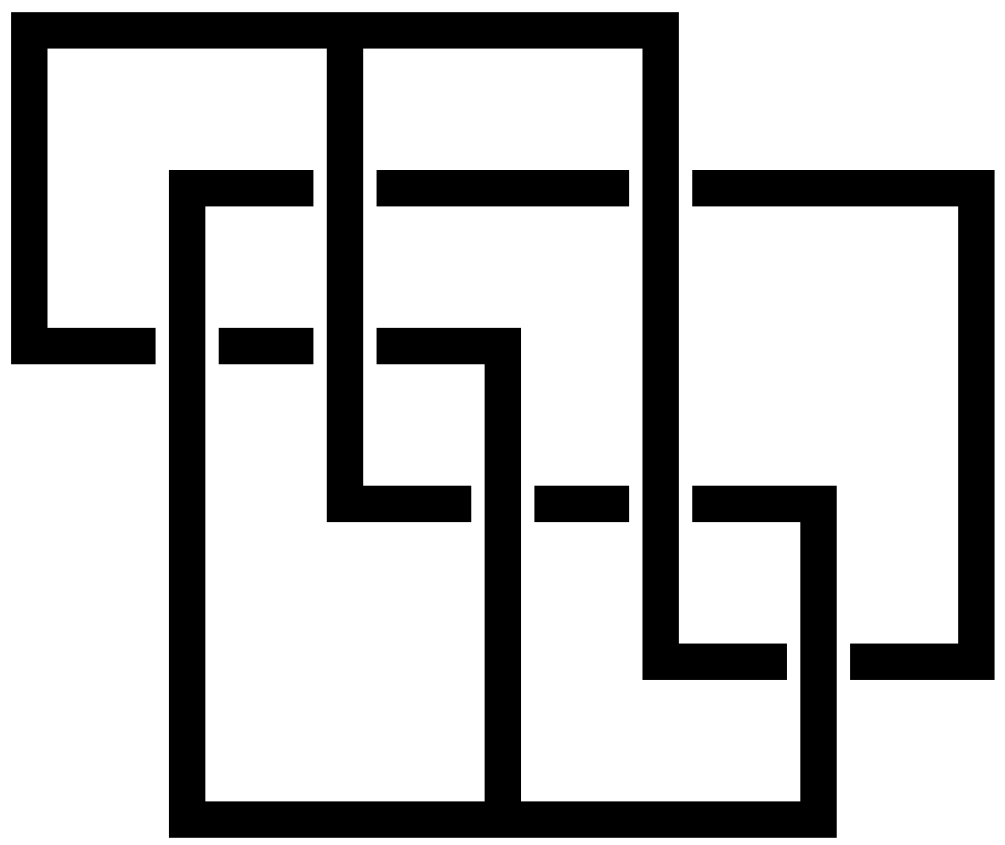
\includegraphics[height=3cm]{figure/exT-shape.png}} &
			$\longmapsto$ &
			\raisebox{-1.5cm}{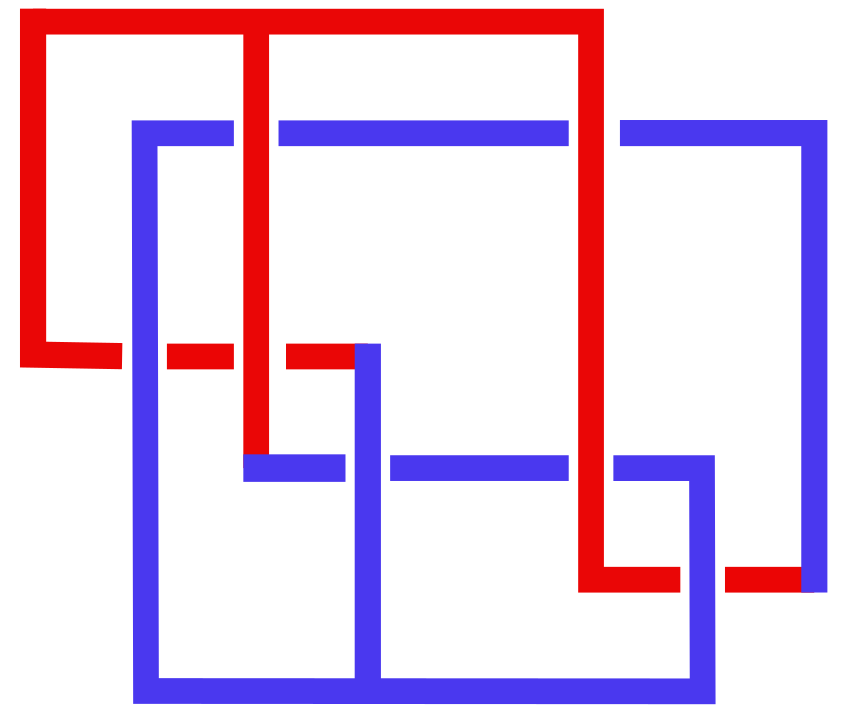
\includegraphics[height=3cm]{figure/T-shape.png}} 
	\end{tabu}
\end{frame}

\begin{frame}
	\begin{enumerate}
		\item[\mybf{CASE 1.}] \mybf{When $M$ represents $\theta$-curve}
	\end{enumerate}
	\mybfff{\circled{i} Line-shape} \\
	\begin{tabu}{X[5c]X[c]X[5c]X[c]X[5c]}
			\raisebox{-1.5cm}{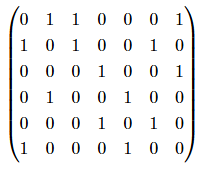
\includegraphics[height=3cm]{figure/L-shape.png}}&
			$\longmapsto$ &
			\raisebox{-1.5cm}{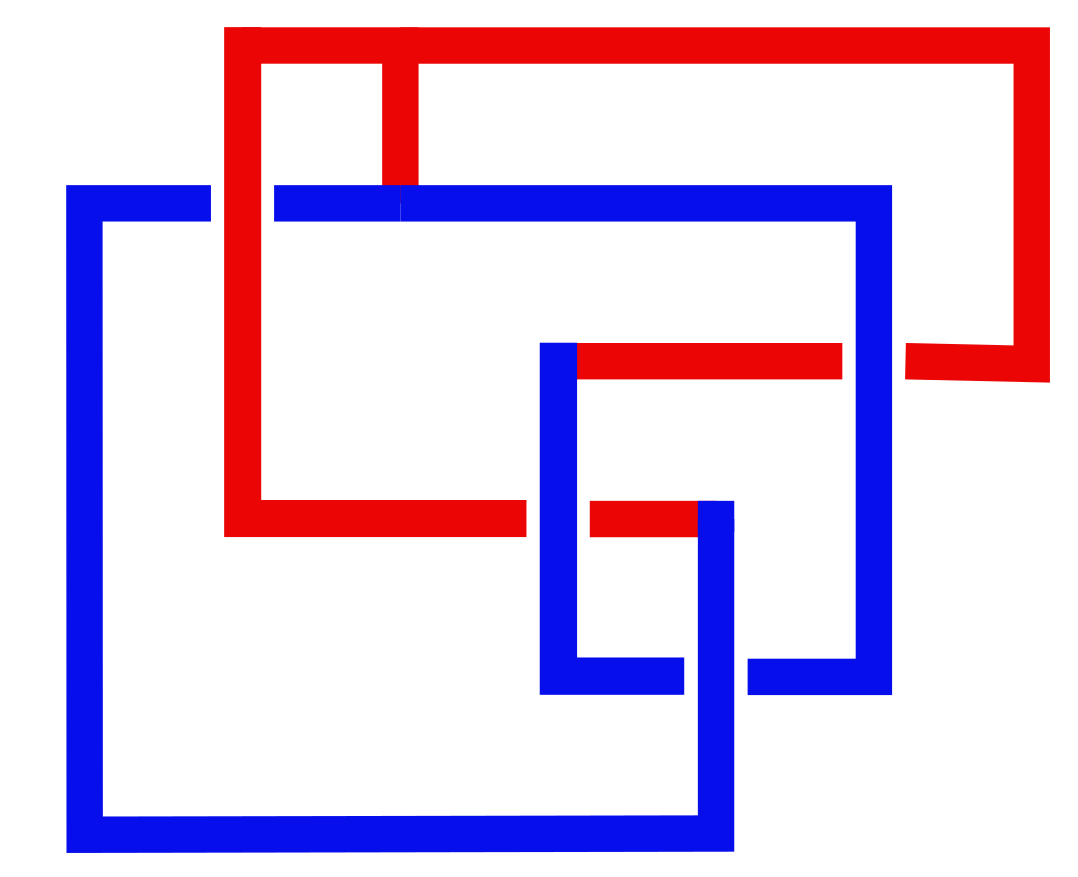
\includegraphics[height=3cm]{figure/Line-shape.png}} &
			$\xmapsto{H-deletion}$ &
			$\begin{bmatrix}
			\textcolor{RoyalBlue}{1} & \textcolor{RoyalBlue}{1} & 0 & 0 & \textcolor{RoyalBlue}{1} \\
			0 & 0 & \textcolor{RoyalBlue}{1} & 0 & 0\\
			0 & 0 & 0 & \textcolor{RoyalBlue}{1} & 0\\
			0 & 0 & \textcolor{RoyalBlue}{1} & 0 & \textcolor{RoyalBlue}{1} \\
			\textcolor{RoyalBlue}{1} & 0 & 0 & \textcolor{RoyalBlue}{1} & 0\\
		\end{bmatrix}$ &
	\end{tabu} \\
	and simplify with
	\begin{tabu}{X[c]X[5c]X[c]X[5c]}
		$\xmapsto[operations]{row/column}$ &
		$\begin{bmatrix}
			\textcolor{RoyalBlue}{1} & 0 & 0 & 0 & 0\\
			\textcolor{RoyalBlue}{1} & \textcolor{RoyalBlue}{1} & 0 & 0 & 0\\
			0 & \textcolor{RoyalBlue}{1} & \textcolor{RoyalBlue}{1} & 0 & \textcolor{RoyalBlue}{1}\\
			0 & 0 & \textcolor{RoyalBlue}{1} & \textcolor{RoyalBlue}{1} & 0\\
			0 & 0 & 0 & \textcolor{RoyalBlue}{1} & 0\\
		\end{bmatrix}$ &
		$\xmapsto{subtracting}$ &
		$\begin{bmatrix}
			\textcolor{red}{1} & 0& 0 & 0 & 0 \\
			0 & \textcolor{red}{1} & 0 & 0 & 0\\
			0 & 0 & \textcolor{red}{1} & 0 & \textcolor{red}{1}\\
			0 & 0 & 0 & \textcolor{red}{1} & \textcolor{red}{-1}\\
			0 & 0 & 0 & 0 & \textcolor{red}{1}\\
		\end{bmatrix}$ 
	\end{tabu}
	So det($M$) = $\pm1$
\end{frame}

\begin{frame}
	\begin{enumerate}
		\item[\mybf{CASE 1.}] \mybf{When $M$ represents $\theta$-curve}
	\end{enumerate}
	\mybfff{\circled{ii} T-shape} \\
	\begin{tabu}{X[5c]X[c]X[5c]X[c]X[5c]}
			$\begin{bmatrix}
			\textcolor{RoyalBlue}{1} & 0 & \textcolor{RoyalBlue}{1} & 0 & \textcolor{RoyalBlue}{1} & 0 & 0\\
			0 & \textcolor{RoyalBlue}{1} & 0 & 0 & 0 & 0 & \textcolor{RoyalBlue}{1}\\
			\textcolor{RoyalBlue}{1} & 0 & 0 & \textcolor{RoyalBlue}{1} & 0 & 0 & 0\\
			0 & 0 & \textcolor{RoyalBlue}{1} & 0 & 0 & \textcolor{RoyalBlue}{1} & 0\\ 
			0 & 0 & 0 & 0 & \textcolor{RoyalBlue}{1} & 0 & \textcolor{RoyalBlue}{1}\\
			0 & \textcolor{RoyalBlue}{1} & 0 & \textcolor{RoyalBlue}{1} & 0 & \textcolor{RoyalBlue}{1} & 0\\
			\end{bmatrix}$&
			$\longmapsto$ &
			\raisebox{-1.5cm}{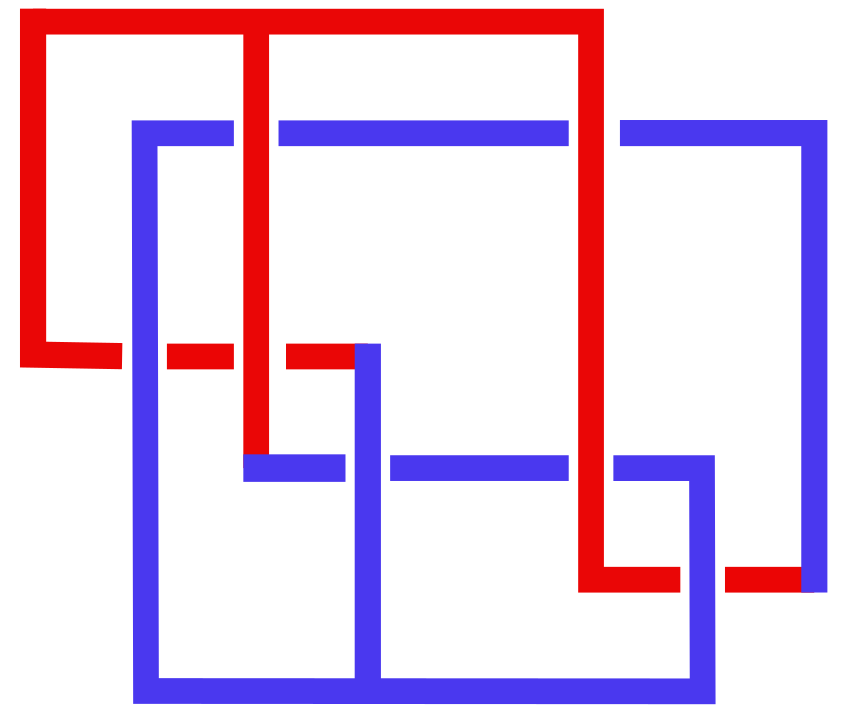
\includegraphics[height=3cm]{figure/T-shape.png}} &
			$\xmapsto{H-deletion}$ &
			$\begin{bmatrix}
			\textcolor{RoyalBlue}{1} & 0 & 0 & 0 & \textcolor{RoyalBlue}{1} \\
			0 & 0 & \textcolor{RoyalBlue}{1} & 0 & 0\\
			0 & \textcolor{RoyalBlue}{1} & 0 & \textcolor{RoyalBlue}{1} & 0\\
			0 & 0 & 0 & 0 & \textcolor{RoyalBlue}{1} \\
			\textcolor{RoyalBlue}{1} & 0 & \textcolor{RoyalBlue}{1} & \textcolor{RoyalBlue}{1} & 0\\
		\end{bmatrix}$ &
	\end{tabu} \\
	and simplify with
	\begin{tabu}{X[c]X[5c]X[c]X[5c]}
		$\xmapsto[operations]{row/column}$ &
		$\begin{bmatrix}
			\textcolor{RoyalBlue}{1} & 0 & 0 & 0 & 0\\
			\textcolor{RoyalBlue}{1} & \textcolor{RoyalBlue}{1} & 0 & \textcolor{RoyalBlue}{1} & 0\\
			0 & \textcolor{RoyalBlue}{1} & \textcolor{RoyalBlue}{1} & 0 & 0\\
			0 & 0 & 0 & \textcolor{RoyalBlue}{1} & \textcolor{RoyalBlue}{1}\\
			0 & 0 & 0 & 0 & \textcolor{RoyalBlue}{1}\\
		\end{bmatrix}$ &
		$\xmapsto{regioning}$ &
		\raisebox{-1.5cm}{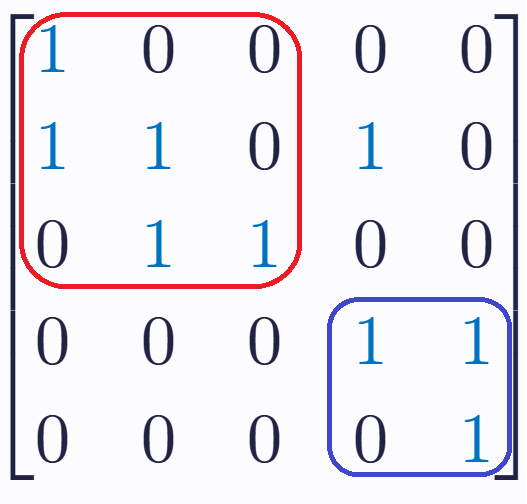
\includegraphics[height=3cm]{figure/regioning.png}}
	\end{tabu}
	So det($M$) = $\pm1$
\end{frame}

